\chapter{Thermal Modeling}

\begin{figure}
\begin{center}
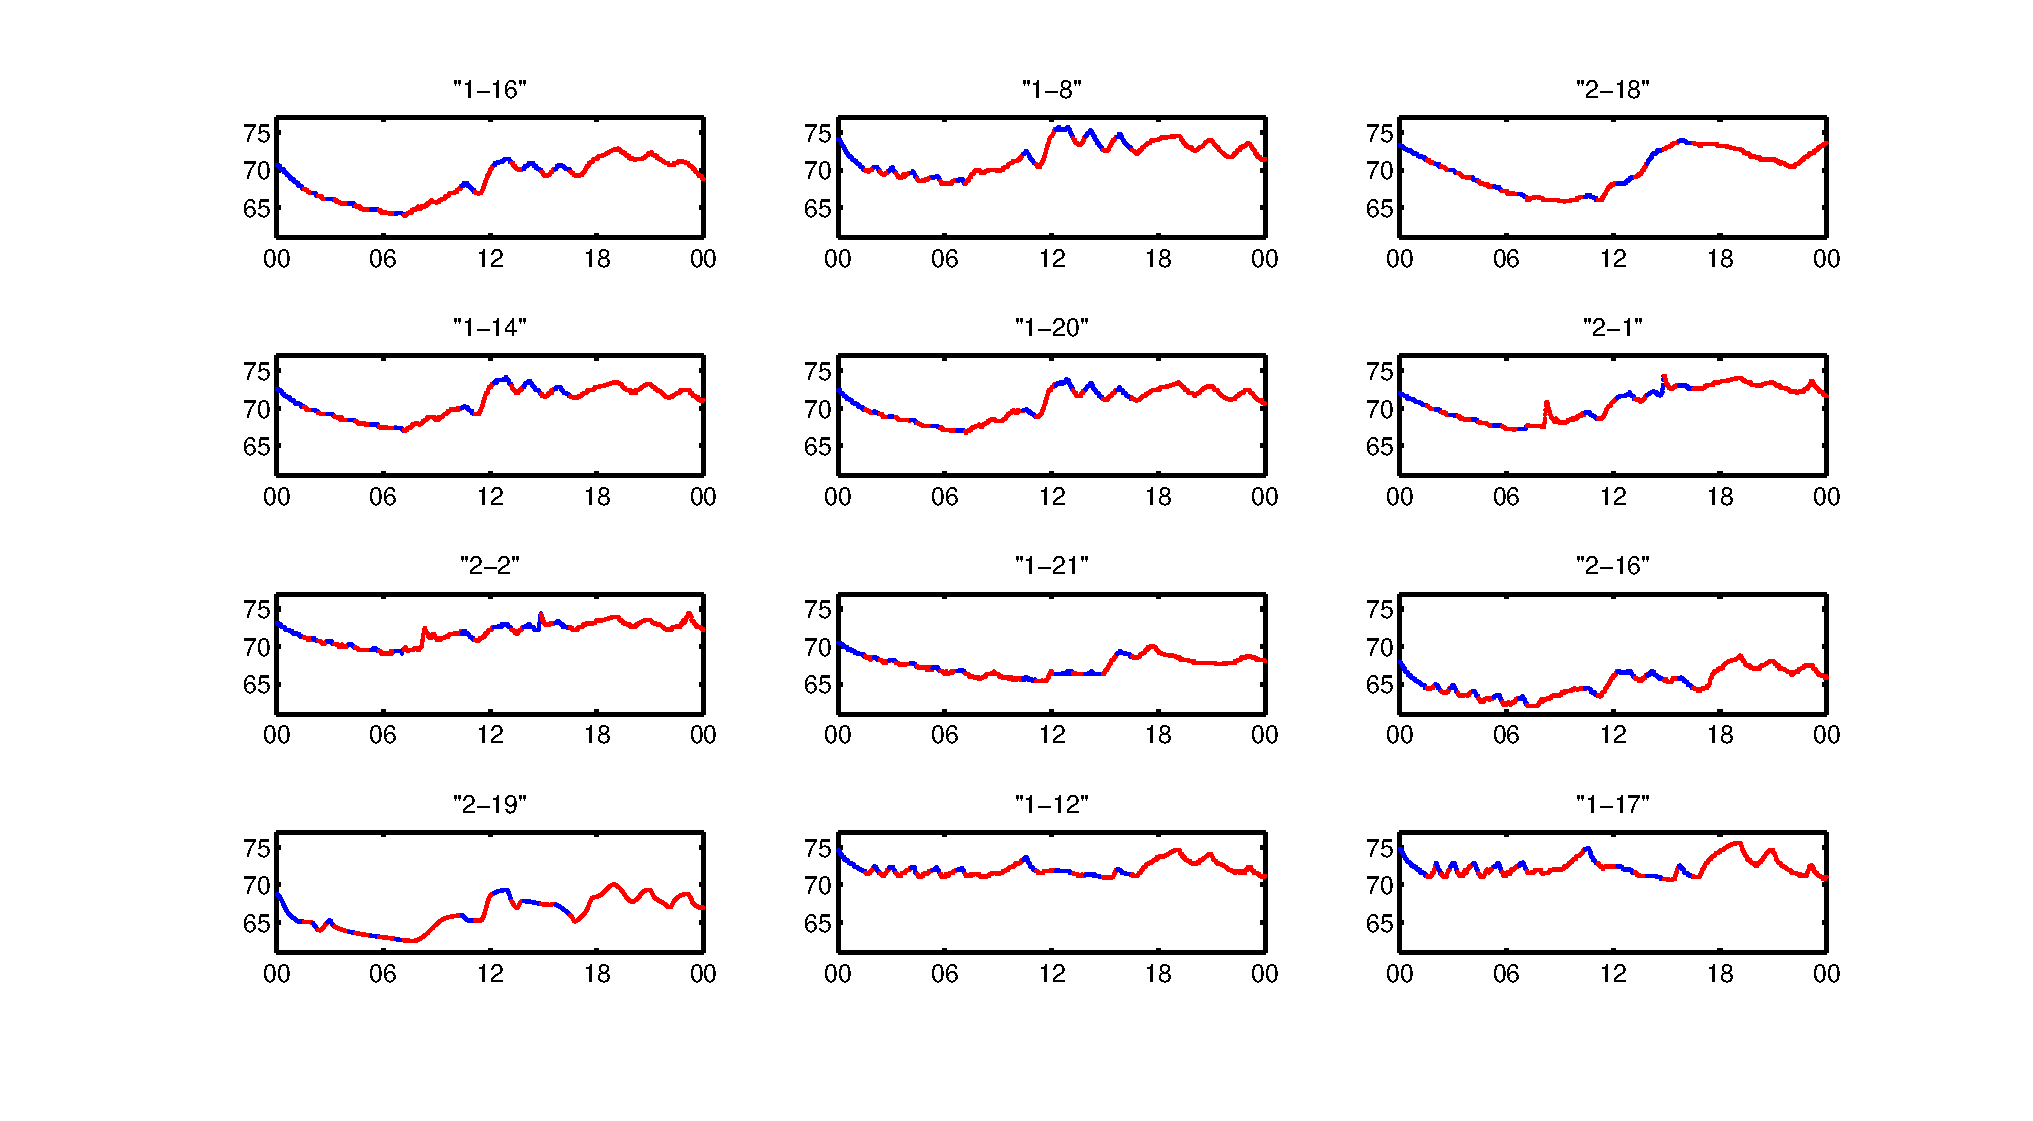
\includegraphics[width=1\columnwidth]{fig/1daytemponoff.eps}
\end{center}
\caption[Effect of HVAC system on temperature sensors]{The effect on temperature
  sensors, within a 24-hour period, of the HVAC system being on (red) and off
  (blue) when heating with all air vent dampers open. The locations of the
  twelve sensors are presented in Figure~\ref{fig:floorplan}}
\label{fig:hvacOnOffAffect}
\end{figure}

We define the problem of thermal modeling as mapping the effect of a set of air
vent dampers {\em D} to a set of temperature sensors {\em T} that are dispersed
across a house (Figure~\ref{fig:floorplan}). The dampers can be opened or
closed, determining if conditioned air is delivered directly into a room. Due to
the lack of thermal isolation between rooms, even if the air vent dampers of a
room are closed, its temperature could still be affected by the HVAC system due
to leakage from neighboring rooms. The temperature sensors monitor the
temperatures at different points throughout the
house. Figure~\ref{fig:hvacOnOffAffect} shows the readings at the twelve
temperature sensors in our deployment during a day with all air vent dampers
open. As the figure shows, the HVAC system being off (blue) causes drops in
temperature while the HVAC system being on (red) usually causes temperature
increases. We are attempting to learn and predict these effects on the
temperature sensors when different sets of air vent dampers are opened and
closed. 

In other words, we want to answer the question {\em ``What effect does each
  register being open have on the reading of each temperature sensor?''}  Being
able to make such a prediction allows us to implement a fine-grained automated
zoning controller that can dynamically alter zones within a single floor to
maintain occupied rooms at a comfortable temperature while allowing unoccupied
rooms to drift. Yet, answering this question is difficult due to the effect of
the weather on the internal temperature of houses. Wind, solar gain, outdoor
temperature, and other weather conditions have a much greater influence on
indoor temperature than the conditioned air provided by an HVAC system. These
weather conditions constantly change, and rarely repeat, therefore including it
as part of a model is impossible without greatly increasing the complexity of
the model. 

But, ignoring the effect of weather on internal temperature makes it impossible
to isolate the effect of a particular register on a temperature sensor. Thus, a
secondary question we are attempting to answer is {\em ``Can we learn the effect
  of dampers on temperature sensors without knowing the weather during the
  training phase?''} In other words, we are attempting to capture the effect of
the weather on the temperature sensor readings while ignoring the actual weather
conditions, such as the external temperature or the position of the sun.

There have been a number of approaches proposed for learning the thermal
response of buildings in order to control HVAC systems
efficiently~\cite{Henze2004,Deng2010,Oldewurtel2010,Ma2011,Nghiem2011,Aswani2011}. Yet,
these approaches require a large amount of data or sophisticated sensors that
will hinder our goal of developing a cheap and easy to install retrofit to
enable room-level zoning of existing centralized HVAC systems.

